\documentclass{report}
\usepackage[margin=1in]{geometry}
\usepackage{graphicx, darkmode, tikz, dsfont, xcolor}
\graphicspath{ {./images/} }

\enabledarkmode{}

% Custom TODO Command
\newcommand{\todotext}[1]{\colorbox{orange}{\textcolor{white}{\textbf{TODO}}}}
\newcommand{\todo}[1]{\textsf{\todotext{} \textcolor{orange}{#1}}}

% Title
\title{Nearest Neighbor Methods}
\author{Aru Gyani\\\small{These notes follow Professor Iyer's slides and are
supplemented with online sources for explanations \& examples.}}
\date{\today}

\begin{document}
\addtolength{\skip\footins}{20pt}
\maketitle
\tableofcontents
\clearpage

\chapter{Introduction}

Imagine a fruit market where fruits are arranged according to their
characteristics like sweetness, color, size, etc.
Now, you come across a fruit you've never seen before, and you want to know whether it's likely to be sweet
or not. To make an \emph{educated guess}, you look around and find the 3 fruits
closest to this mysterious one, a.k.a it's \textbf{nearest neighbors}. You
notice that 2 out of 3 (a majority) of these fruits are sweet. Based on this, you can
reasonably predict that the mysterious fruit is sweet as well. This is the essence of nearest neighbor methods. 

\section{General Description}
For nearest neighbor methods (kNN), the learning phase involves storing all training
examples. This is different than regression where the data is split into
\emph{train} and \emph{test} sets. To classify a point, \(x'\) with kNN methods, we find
the k-data points, \((x^{(i)}, y^{(i)})\), such that \(x^{(i)}\) (feature
vector) is closest to \(x'\). 
\\[12pt]
We preedict the label \(y'\) of a new data point \(x'\) to be the most frequent
label among its \(k\) nearest neighboring data points in the training dataset,
a.k.a a majority vote.

\section{Characteristics}
Nearest neighbor methods apply to data sets with points in \(\mathds{R}^d\).
  \begin{itemize}
    \item This means that these methods apply to datasets where each
    data point is a vector of \(d\) real-valued\footnote{The term ``real-valued''
    is used here as a generalizationn for the type of data, since it could be
    phsyical measurements, probabilities, monetary values, etc.} features.
    \item Best for large data sets with only a few (\(< 20\)) attributes.
  \end{itemize}

\subsection{Advantages}
  \begin{itemize}
    \item \emph{Learning is easy.}
    
    With nearest neighbor methods, learning is considered ``easy'' for a few
    reasons. First, there is no ``training phase'' where we have to fit a model
    to the data. Here, we simply are storing the dataset.
    \\[12pt]
    Also, the model is quite versatile when it comes to its use-case. For
    \textbf{classification}, we predict labels by majority voting and for
    \textbf{regression} we predict labels by averaging.

    \item \emph{Can learn complicated decision boundaries.}
    
    This means that we are not limited by situations where the separation
    between classes in the data is not linear or curved. Instead, the
    decision boundary can be non-linear, curved, or even have zigzag lines and
    more complex shapes.
  \end{itemize}

\subsection{Disadvantages}
  \begin{itemize}
    \item \emph{Classification is slow} (need to keep the entire training set around).
    \item \emph{Easily fooled by irrelevant attributes.}
    
    With nearest neighbor methods, we tend to consider all attributes or
    features provided to us, without distinguishing between those that are
    relevant or not. This makes the method susceptible to noisy data,
    overfitting, computational complexity, and more.
  \end{itemize}
  \begin{figure}[h!]
    \centering
    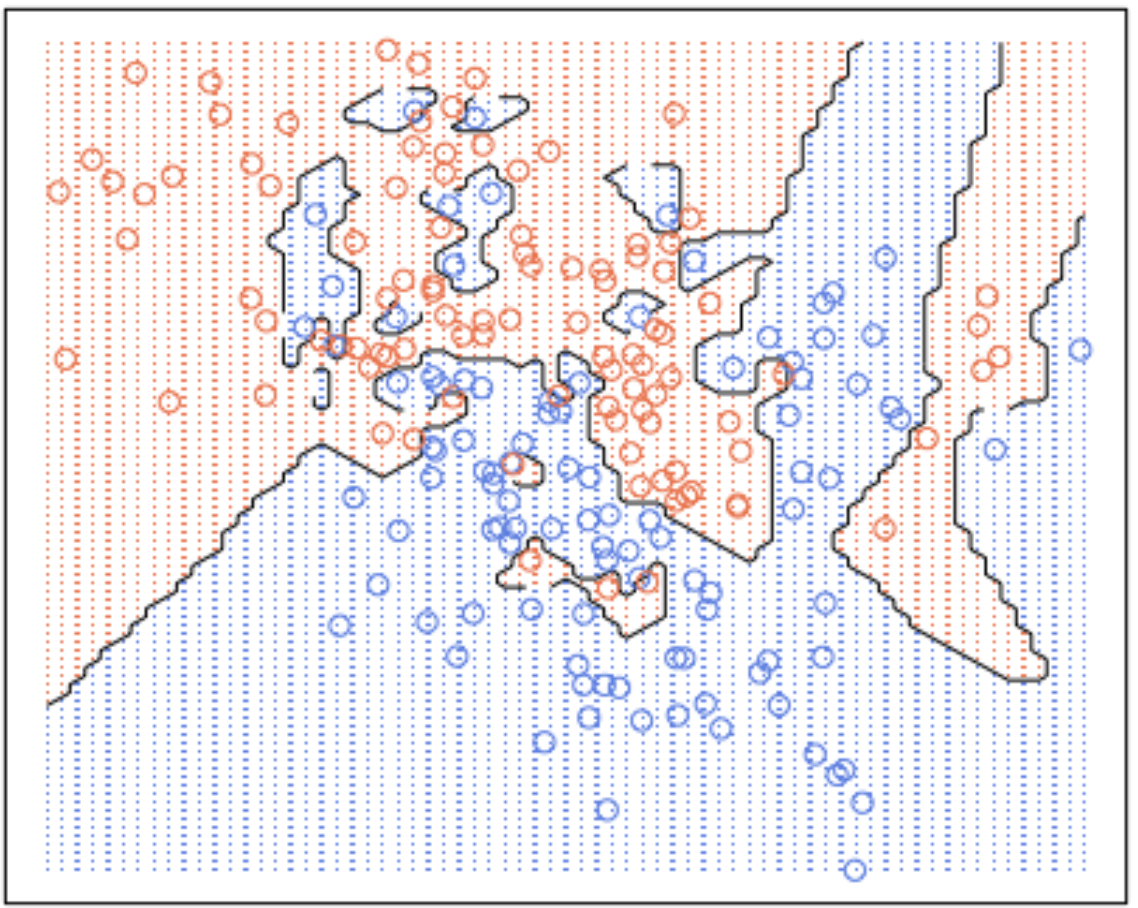
\includegraphics[width=7.5cm]{1nn.png}
    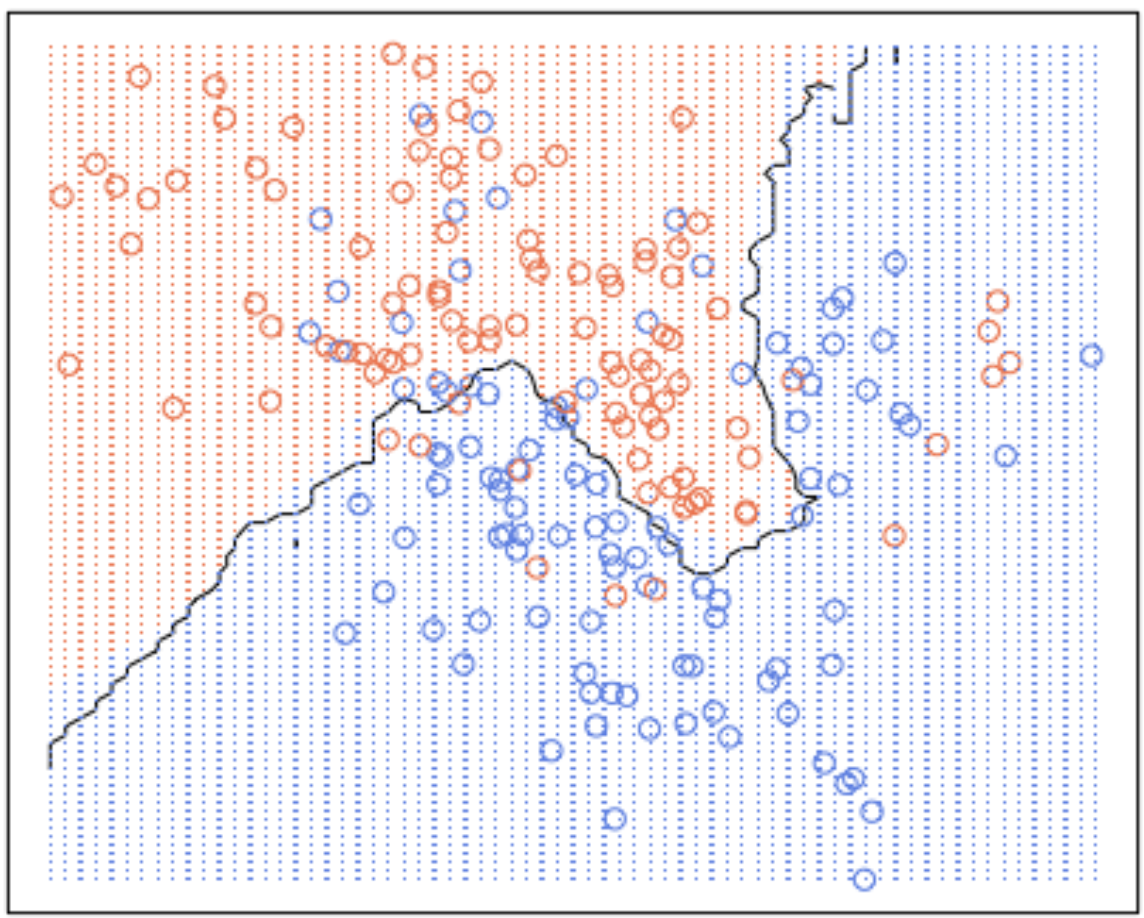
\includegraphics[width=7.5cm]{20nn.png}
    \caption{kNN classification when \(k\) (nearest neighbors to include) = 1 (left) and 20 (right)}
  \end{figure}
  When observing Figure 1, there are a few interest things to note. 
  \begin{itemize}
    \item When \(k = 1\), the classifications are very specific to each data point
    and have small pockets of different classes within larger regions. 
    \item When \(k = 20\), the decision boundary is more flexible and ends up misclassifying
    some data points.
    \begin{quote}
      Question for TA: Is this necessarily good or bad? Is it possible this data
      is just noisy and with \(k = 20\) it's actually able to ``ignore'' the noise.
    \end{quote}
    \begin{quote}
      Note to self: Might be helpful to try re-creating some of these plots to get a
      better intuition.
    \end{quote}
  \end{itemize}

\section{Practical Challenges}
The following are challenges faced when using the kNN methods.
\begin{itemize}
  \item How do we choose the right measure of closeness?
  
  Euclidean distance is the most popular formula for calculating distance, but
  there are many other possibilities. Euclidean distance makes sense
  when each of the features is \textbf{roughly on the same scale}.

  \todo{Ask TA about formula when using feature vectors.}

  \item How do we pick the right value for \(k\)?
  \item What if the nearest neighbor is really far away?
\end{itemize}

\end{document}